\thispagestyle{thachthuctoanhocnone}
\pagestyle{thachthuctoanhoc}
\everymath{\color{thachthuctoanhoc}}
\graphicspath{{../thachthuctoanhoc/pic/}}
\begingroup
\AddToShipoutPicture*{\put(0,616){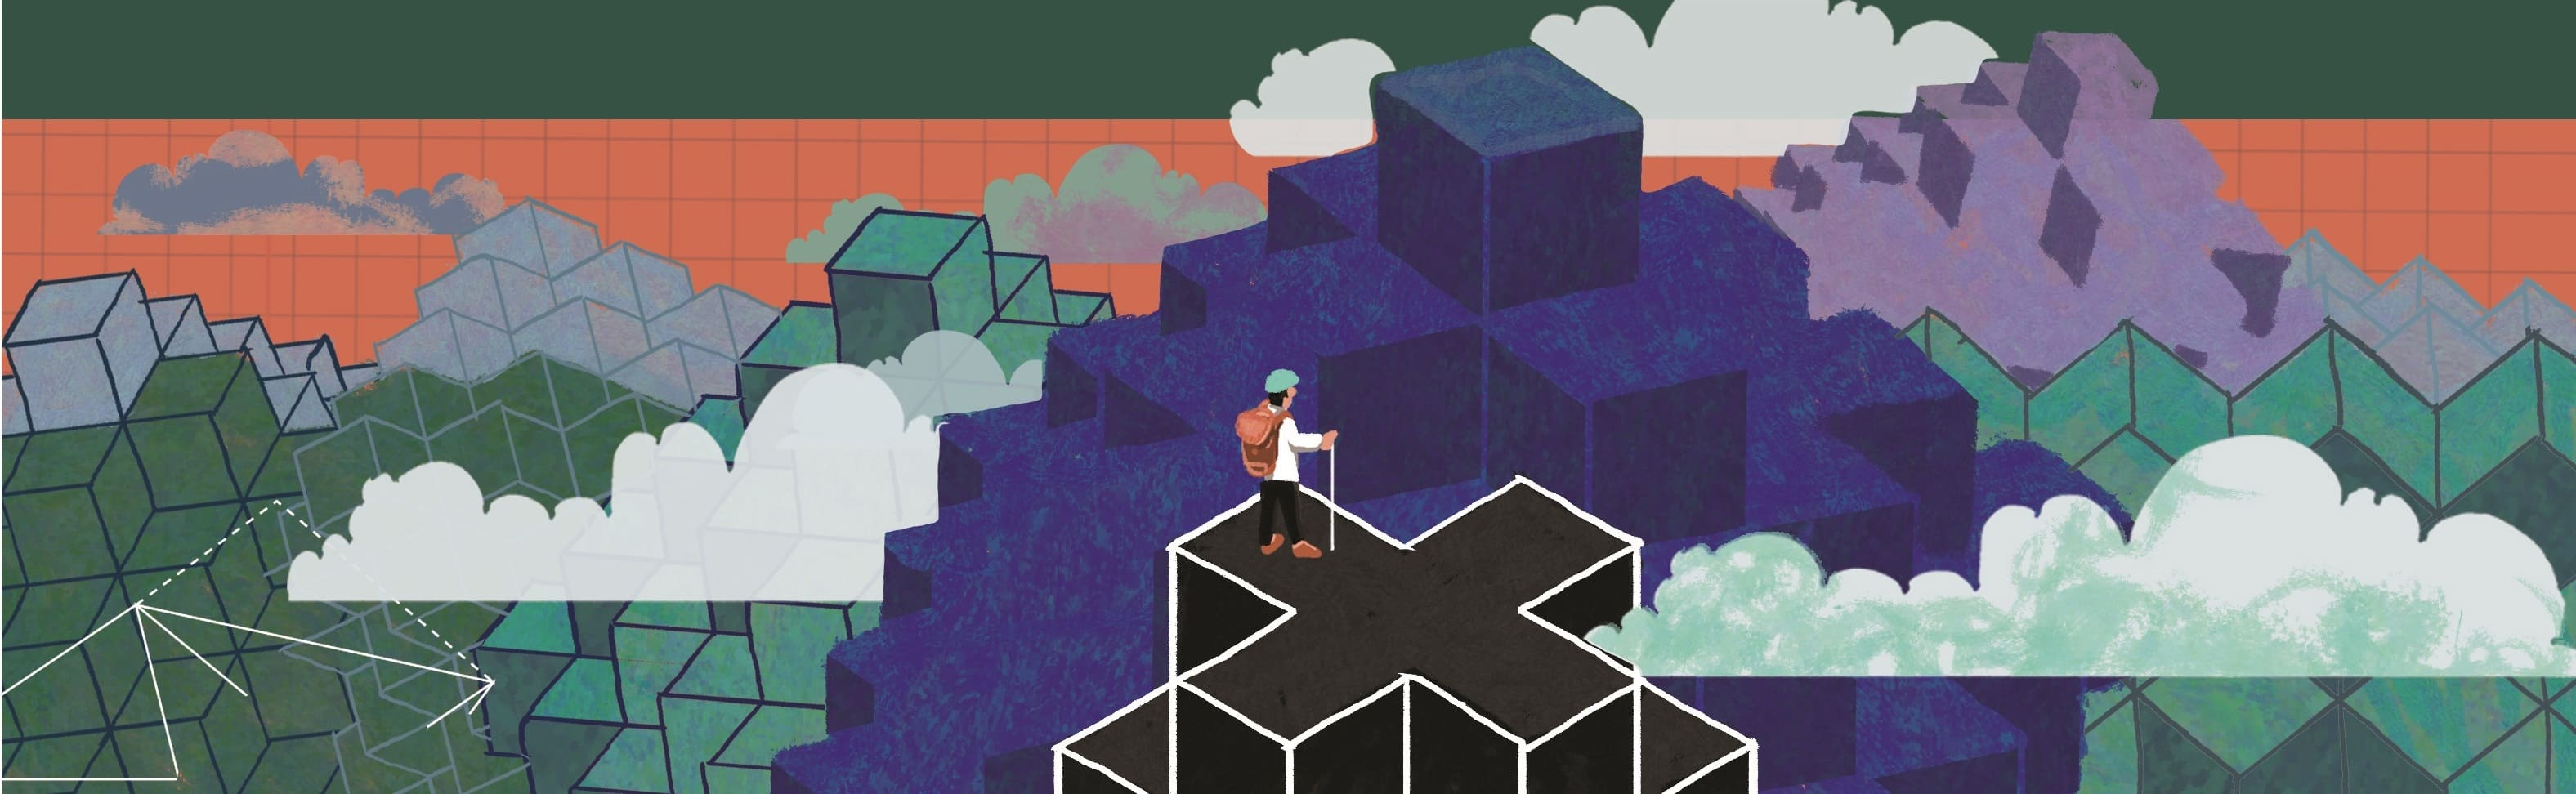
\includegraphics[width=19.3cm]{../thachthuctoanhoc/bannerthachthuc}}}
\centering
\vspace*{4cm}
\endgroup
\vspace*{-8pt}
\begin{tBox}
	\begin{itemize}[leftmargin = 13pt, itemsep = 1.0pt] 
		\item Mỗi bài toán đề xuất (kèm theo lời giải) cần được nêu rõ là bài sáng tác hay bài sưu tầm.
		%		\item Mỗi bài toán đề xuất (kèm theo lời giải) cần được nêu rõ là bài sáng tác hay bài sưu tầm (nếu là bài sưu tầm, cần ghi rõ nguồn).
		\item Bài giải cho mỗi bài toán cần được trình bày trong một file riêng hoặc
		một tờ giấy riêng.
		\item  Người đề xuất bài toán hoặc gửi bài giải cho các bài toán trong mục ``Thách thức kỳ này" cần ghi rõ họ, đệm, tên và nơi làm việc/học tập, số điện thoại liên hệ. Nếu là học sinh (hoặc sinh viên) cần ghi rõ là học sinh lớp mấy (hoặc sinh viên năm thứ mấy).
		\item Các bài toán trong mục Thách thức kỳ này hướng tới các độc giả là học sinh phổ thông; được phân chia thành các mức độ $B$, $A$, và được sắp xếp theo độ khó tăng dần, theo đánh giá chủ quan của Ban biên tập. Các bài toán mức độ $B$ không đòi hỏi các kiến thức vượt quá chương trình môn Toán cấp THCS; các bài toán mức độ $A$ không đòi hỏi các kiến thức vượt quá chương trình môn Toán cấp THPT.
		\item Cách thức gửi bài toán đề xuất hoặc lời giải: gửi file thu được bằng cách scan, ảnh chụp (rõ nét) của bản viết tay, hoặc được soạn thảo bằng các phần mềm Latex, Word tới \url{bbt@pi.edu.vn} hoặc gửi qua đường bưu điện tới Tòa soạn (xem địa chỉ tại bìa $2$).
		\item Hạn gửi lời giải cho các bài toán P$751$--P$760$: trước ngày $15/12/2023$.
	\end{itemize}
\end{tBox}
\begin{center}
	\vspace*{-5pt}
	\textbf{\color{thachthuctoanhoc}\color{thachthuctoanhoc}\color{thachthuctoanhoc}\color{thachthuctoanhoc}\color{thachthuctoanhoc}THÁCH THỨC KỲ NÀY}
	\vspace*{-5pt}
\end{center}
\begin{multicols}{2}
	\setlength{\abovedisplayskip}{4pt}
	\setlength{\belowdisplayskip}{4pt}
	{\color{thachthuctoanhoc}{\usefont{T5}{qag}{b}{n} P751.}}
	(Mức $B$) Người ta ghép khít năm hình chữ nhật bằng nhau với nhau, để được một hình dài $27$cm và rộng $15 $cm, như ở hình vẽ dưới đây. Biết rằng, đoạn thẳng $A C$ chia hình đó thành hai phần có diện tích bằng nhau. Hãy tính độ dài đoạn thẳng $A B$.
	\begin{figure}[H]
		\vspace*{-10pt}
		\centering
		\captionsetup{labelformat= empty, justification=centering}
		\definecolor{qqqqff}{rgb}{0,0,1}
		\begin{tikzpicture}[scale=0.48,thachthuctoanhoc, node font=\small]
			\draw  (-4,2)-- (-4,-2);
			\draw  (-4,-2)-- (-0.42,-2);
			\draw  (-0.42,-2)-- (-0.42,4);
			\draw  (-4,2)-- (6.74,2);
			\draw  (6.74,2)-- (6.74,4);
			\draw  (6.74,4)-- (-0.42,4);
			\draw  (3.16,4)-- (3.16,0);
			\draw  (3.16,0)-- (-4,0);
			\draw  (-4,-2)-- (4.5,4);
			\draw[decoration={brace,mirror,raise=5pt},decorate]
			(-4,-3) -- node[below = 6pt] {$27\text{ cm}$} (6.74,-3);
			\draw[decoration={brace,mirror,raise=5pt},decorate]
			(-4.5,4) -- node[left = 5pt] {$15\text{ cm}$} (-4.5,-2);
			\draw [fill=white] (-4,-2) circle (1.5pt);
			\draw (-4.08,-2.52) node {$C$};
			\draw [fill=white] (6.74,4) circle (1.5pt);
			\draw (6.74,4.5) node {$B$};
			\draw [fill=white] (4.5,4) circle (1.5pt);
			\draw (4.5,4.5) node {$A$};
		\end{tikzpicture}
		\vspace*{-10pt}
	\end{figure}
	\begin{flushright}
		\textit{Đăng Hải, Hà Nội (st)}
	\end{flushright}
	{\color{thachthuctoanhoc}{\usefont{T5}{qag}{b}{n} P752.}}
	(Mức $B$) Cho $x,y,z$ là các số thực thoả mãn 
	\begin{align*}
		x^2y+y^2z+z^2x=1 \text{ và } xy^2+yz^2+zx^2=2.
	\end{align*}
	 Tính giá trị của biểu thức
	\begin{align*}
		P=\left(\!x^2\!+\!xy\!+\!y^2\!\right)\!\left(\!y^2\!+\!yz\!+\!z^2\!\right)\!\left(\!z^2\!+\!zx\!+\!x^2\!\right).
	\end{align*}
	\begin{flushright}
		\textit{Trần Quốc Luật, Tp. Hồ Chí Minh}
	\end{flushright}
	{\color{thachthuctoanhoc}{\usefont{T5}{qag}{b}{n} P753.}}
	(Mức $B$) Cho đường tròn $(O)$ với đường kính $AB = 2R$. Gọi $C$ là trung điểm của $OA$. $M$ là một điểm nằm trên $(O)$. Đường thẳng $MC$ cắt $(O)$ tại điểm thứ hai $D$.  Đường thẳng qua $D$ và vuông góc với $AB$ cắt $(O)$ tại điểm thứ hai $E$. Đường thẳng $ME$ cắt đường thẳng $AB$ tại điểm $F$. Tìm vị trí của điểm $M$  sao cho tổng $EF + MC$ có giá trị nhỏ nhất.
	\begin{figure}[H]
%		\vspace*{5pt}
		\centering
		\captionsetup{labelformat= empty, justification=centering}
		\definecolor{qqwuqq}{rgb}{0.,0.39215686274509803,0.}
		\definecolor{uuuuuu}{rgb}{0.26666666666666666,0.26666666666666666,0.26666666666666666}
		\definecolor{xdxdff}{rgb}{0.49019607843137253,0.49019607843137253,1.}
		\definecolor{ududff}{rgb}{0.30196078431372547,0.30196078431372547,1.}
		\begin{tikzpicture}[thachthuctoanhoc,scale=0.85]
			\draw[color=qqwuqq,fill=qqwuqq,fill opacity=0.10000000149011612] (-1.5617418181909823,1.) -- (-1.5617418181909823,1.1880461622337974) -- (-1.7497879804247796,1.1880461622337974) -- (-1.7497879804247796,1.) -- cycle; 
			\draw  (0.,1.) circle (2.cm);
			\draw  (-2.,1.)-- (2.,1.);
			\draw  (-4.,1.)-- (0.4991521613769648,2.936710386142622);
			\draw  (0.4991521613769648,2.936710386142622)-- (-1.7497879804247796,0.03137105991975908);
			\draw  (-2.,1.)-- (-4.,1.);
			\draw  (-1.7497879804247796,1.968628940080241)-- (-1.7497879804247796,0.03137105991975908);
				\draw [fill=white] (0.,1.) circle (1.5pt);
				\draw (0.09082211690268885,1.2491318135923188) node {$O$};
				\draw [fill=white] (-2.,1.) circle (1.5pt);
				\draw (-2.2228335500515635,0.7335225357666101) node {$A$};
				\draw [fill=white] (2.,1.) circle (1.5pt);
				\draw (2.2449153240669926,0.9831943806090713) node {$B$};
				\draw [fill=white] (-1.,1.) circle (1.5pt);
				\draw (-1.0793025882235996,1.2757255568906436) node {$C$};
				\draw [fill=white] (0.4991521613769648,2.936710386142622) circle (1.5pt);
				\draw (0.6492907261675084,3.2170688176683497) node {$M$};
				\draw [fill=white] (-1.7497879804247796,0.03137105991975908) circle (1.5pt);
				\draw (-1.9435992454191537,-0.1869303245172173) node {$D$};
				\draw [fill=white] (-1.7497879804247796,1.968628940080241) circle (1.5pt);
				\draw (-1.917005502120829,2.233100315630334) node {$E$};
				\draw [fill=white] (-4.,1.) circle (1.5pt);
				\draw (-4.00461435103932,0.67413058716358) node {$F$};
		\end{tikzpicture}
		\vspace*{-10pt}
	\end{figure}
	\vskip 0.05cm
	\hfill \textit{Trần Thanh Hưng, Phú Yên}
	\vskip 0.05cm
	{\color{thachthuctoanhoc}{\usefont{T5}{qag}{b}{n} P754.}}
	(Mức $B$) Cho $a, b, c$ là các số thực dương. Chứng minh rằng
	\begin{align*}
		&\frac{b+c}{\sqrt{\!a^2\!+\!b c}\!+\!\!\sqrt{\!a(b+c)}}\!+\!\frac{c\!+\!a}{\sqrt{\!b^2\!+\!c a}\!+\!\!\sqrt{\!b(c\!+\!a)}}\\
		&+\frac{a+b}{\sqrt{c^2+a b}+\sqrt{c(a+b)}} \geq \frac{3}{\sqrt{2}} .
	\end{align*}
	\vskip 0.05cm
	\hfill	\textit{Nguyễn Việt Hùng, Hà Nội}
	\vskip 0.05cm
	{\color{thachthuctoanhoc}{\usefont{T5}{qag}{b}{n} P755.}}
	(Mức $B$) Trong một hình chữ nhật có kích thước $10\times 5$, lấy $1351$ điểm đôi một phân biệt tuỳ ý. Chứng minh rằng, tồn tại một hình tròn bán kính bằng $\dfrac14$ chứa ít nhất $4$ điểm trong số các điểm đã lấy.
	\vskip 0.05cm
	\hfill	\textit{Phạm Nhật Nguyệt, Hải Phòng (st)}
	\vskip 0.05cm
	{\color{thachthuctoanhoc}{\usefont{T5}{qag}{b}{n} P756.}}
	(Mức $B$) Ta gọi số nguyên dương $n$ là ``số đẹp" nếu trong $22$ số: $5,n+5,2n+5,\ldots,21n+5$, tồn tại một số có cùng số dư với tích tất cả các số đó, trong phép chia cho $23$. Hãy tìm tất cả các số đẹp.
	\vskip 0.05cm
	\hfill	\textit{Hà Duy Hưng, Hà Nội}
	\vskip 0.05cm
	{\color{thachthuctoanhoc}{\usefont{T5}{qag}{b}{n} P757.}}
	(Mức $A$) Với mỗi số nguyên dương $n$, ký hiệu $a_n$ là nghiệm thực lớn nhất của phương trình
	\begin{align*}
		x^{2023}-nx^{2022}-nx^{2021}-\cdots-nx+1=0.
	\end{align*}
	Xác định tất cả các số thực $C$, để 
	\begin{align*}
		a_1+\cdots+a_n>C. n^2
	\end{align*}
	với mọi số nguyên dương $n$.
	\vskip 0.05cm
	\hfill	\textit{Tô Trung Hiếu, Nghệ An}
	\vskip 0.05cm
	{\color{thachthuctoanhoc}{\usefont{T5}{qag}{b}{n} P758.}}
	(Mức $A$) Tìm số thực $k$ lớn nhất sao cho: 
	\begin{align*}
		a+b+c-3\ge k(a-b)(b-c)(c-a)
	\end{align*}
	với mọi số thực không âm $a,b,c$ thoả mãn $ab+bc+ca=3$. 
	\vskip 0.05cm
	\hfill\textit{Đinh Bình Dương, Hà Nội}
	\vskip 0.05cm
	{\color{thachthuctoanhoc}{\usefont{T5}{qag}{b}{n} P759.}}
	(Mức $A$) Cho tam giác  $ABC$ nội tiếp đường tròn $(O)$, có các đường cao $BE,CF$ cắt nhau tại $H$.  Gọi $M, N$ tương ứng là trung điểm của $AH, EF$. Gọi $P$ là điểm đối xứng với $N$ qua $BC$. Chứng minh rằng
	\begin{align*}
		\angle BMP =\angle NMC. 
	\end{align*}
	\begin{figure}[H]
		\vspace*{-15pt}
		\centering
		\captionsetup{labelformat= empty, justification=centering}
		\definecolor{qqwuqq}{rgb}{0,0.39215686274509803,0}
		\definecolor{ffqqqq}{rgb}{1,0,0}
		\definecolor{qqzzcc}{rgb}{0,0.6,0.8}
		\definecolor{qqqqff}{rgb}{0,0,1}
		\definecolor{qqqqffa}{rgb}{1,1,1}
		\begin{tikzpicture}[thachthuctoanhoc,scale=0.65]
			\draw [shift={(-2.4,1.2974770642201836)},color=qqwuqq] (0,0) -- (-115.88356340862376:0.6) arc (-115.88356340862376:-85.3246079752399:0.6) -- cycle;
			\draw [shift={(-2.4,1.2974770642201836)},color=qqwuqq] (0,0) -- (-70.77370689221246:0.6) arc (-70.77370689221246:-40.2147514588286:0.6) -- cycle;
			\draw (-0.592637676575393,0.4382959745607279) -- (-0.4280391340195052,0.20828006252750003) -- (-0.19802322198627734,0.37287860508338777) -- (-0.3626217645421651,0.6028945171166157) -- cycle; 
			\draw (-3.6432538877850886,-0.7848335552679585) -- (-3.3718647339119383,-0.8645074353041129) -- (-3.292190853875784,-0.5931182814309623) -- (-3.5635800077489344,-0.5134444013948081) -- cycle; 
			\draw [color=qqzzcc] (-2.4,3.45)-- (-4,-2);
			\draw [color=qqzzcc] (-4,-2)-- (1.5,-2);
			\draw [color=qqzzcc] (1.5,-2)-- (-2.4,3.45);
			\draw [color=ffqqqq] (-1.25,0.15252293577981646) circle (3.492256432316814cm);
			\draw  (-2.4,3.45)-- (-2.4,-0.855045871559633);
			\draw  (-3.5635800077489344,-0.5134444013948081)-- (-0.3626217645421651,0.6028945171166157);
			\draw  (-4,-2)-- (-0.3626217645421651,0.6028945171166157);
			\draw  (-3.5635800077489344,-0.5134444013948081)-- (1.5,-2);
			\draw  (-1.9631008861455497,-4.044725057860903)-- (-1.9631008861455497,0.044725057860903805);
			\draw  (-1.9631008861455497,0.044725057860903805)-- (-2.4,1.2974770642201836);
			\draw  (-2.4,1.2974770642201836)-- (1.5,-2);
			\draw  (-4,-2)-- (-2.4,1.2974770642201836);
			\draw  (-2.4,1.2974770642201836)-- (-1.9631008861455497,-4.044725057860903);
			\draw [shift={(-2.4,1.2974770642201836)},color=qqwuqq] (-115.88356340862376:0.6) arc (-115.88356340862376:-85.3246079752399:0.6);
			\draw[color=qqwuqq] (-2.4993715787134962,0.766699060395621) -- (-2.5214541517609392,0.6487483928790517);
			\draw [shift={(-2.4,1.2974770642201836)},color=qqwuqq] (-70.77370689221246:0.6) arc (-70.77370689221246:-40.2147514588286:0.6);
			\draw[color=qqwuqq] (-2.094095810427579,0.8524797307427333) -- (-2.026117101633708,0.7535914344144113);
			\draw [fill=white] (-2.4,3.45) circle (1.5pt);
			\draw (-2.6,4.04) node {$A$};
			\draw [fill=white] (-4,-2) circle (1.5pt);
			\draw (-4.32,-2.26) node {$B$};
			\draw [fill=white] (1.5,-2) circle (1.5pt);
			\draw (1.7,-2.2) node {$C$};
			\draw [fill=white] (-0.3626217645421651,0.6028945171166157) circle (1.5pt);
			\draw (-0.2,0.92) node {$E$};
			\draw [fill=white] (-3.5635800077489344,-0.5134444013948081) circle (1.5pt);
			\draw (-3.94,-0.52) node {$F$};
			\draw [fill=white] (-2.4,-0.855045871559633) circle (1.5pt);
			\draw (-2.5,-1.22) node {$H$};
			\draw [fill=white] (-1.9631008861455497,0.044725057860903805) circle (1.5pt);
			\draw (-1.76,-0.15) node {$N$};
			\draw [fill=white] (-2.4,1.2974770642201836) circle (1.5pt);
			\draw (-1.8,1.68) node {$M$};
			\draw [fill=white] (-1.9631008861455497,-4.044725057860903) circle (1.5pt);
			\draw (-2,-4.36) node {$P$};
		\end{tikzpicture}
		\vspace*{-15pt}
	\end{figure} 
	\vskip 0.01cm
	\hfill	\textit{Lưu Công Đông, Hà Nội}
	\vskip 0.05cm
	{\color{thachthuctoanhoc}{\usefont{T5}{qag}{b}{n} P760.}}
	(Mức $A$) Cho dãy số $(x_n)$ xác định bởi $x_1=4$ và 
	\begin{align*}
			x_{n+1}=45x_n+\sqrt{2024x_n^2+16}
	\end{align*}
	với mọi số nguyên dương $n$.
	\vskip 0.1cm
	Tìm tất cả các số nguyên $a$ sao cho $a^n\left(\dfrac{x_{2n}}{x_n}+2\right)$ là số chính phương, với mọi số nguyên dương $n$.
	\vskip 0.05cm
	\hfill	\textit{Nguyễn Đức Khải, Nam Định}
	\vskip 0.15cm
	\textbf{\color{thachthuctoanhoc}ĐÍNH CHÍNH}
	\vskip 0.1cm
	Do sơ suất trong chế bản đề bài {\color{thachthuctoanhoc}{\usefont{T5}{qag}{b}{n} P727}} đăng trong số $7-8$ bị thiếu điều kiện. Đề bài đúng là như sau:
	\vskip 0.1cm
	Cho số nguyên $k\ge3$. Xét các số thực không âm $x,y,z$ thoả mãn $x+y+z\le 1$. Tìm giá trị lớn nhất của biểu thức
	\begin{align*}
		P=&x^k\left(y^{k-1}+z^{k-1}\right)+y^k\left(z^{k-1}+x^{k-1}\right)\\
		&+z^k\left(x^{k-1}+y^{k-1}\right).
	\end{align*}
	Lời giải sẽ được công bố trong số sau. Thành thật cáo lỗi cùng bạn đọc và tác giả.
\end{multicols}
\newpage
\centerline{{\large{\textbf{\color{thachthuctoanhoc}\color{thachthuctoanhoc}\color{thachthuctoanhoc}GIẢI BÀI KỲ TRƯỚC}}}}
\vspace*{-5pt}
\begin{multicols}{2}
	\setlength{\abovedisplayskip}{5pt}
	\setlength{\belowdisplayskip}{5pt}
	{\color{thachthuctoanhoc}{\usefont{T5}{qag}{b}{n} P731.}}
	(Mức $B$) Ghép chín hình vuông thành một hình chữ nhật, như ở hình dưới đây. Biết rằng, hình vuông màu đen có cạnh bằng $1$. Tìm chiều dài và chiều rộng của hình chữ nhật.
	\begin{figure}[H]
		\vspace*{-5pt}
		\centering
		\captionsetup{labelformat= empty, justification=centering}
		\begin{tikzpicture}[thachthuctoanhoc,scale=0.15]
			\draw[fill=black] (0,0) rectangle (1,1);
			\draw  (0.,-9.)-- (9.,-9.);
			\draw  (9.,-9.)-- (9.,0.);
			\draw  (9.,0.)-- (0.,0.);
			\draw  (0.,0.)-- (0.,-9.);
			\draw  (1.,0.)-- (9.,0.);
			\draw  (9.,0.)-- (9.,8.);
			\draw  (9.,8.)-- (1.,8.);
			\draw  (1.,8.)-- (1.,0.);
			\draw  (-10.,-9.)-- (0.,-9.);
			\draw  (0.,-9.)-- (0.,1.);
			\draw  (0.,1.)-- (-10.,1.);
			\draw  (-10.,1.)-- (-10.,-9.);
			\draw  (-6.,1.)-- (1.,1.);
			\draw  (1.,1.)-- (1.,8.);
			\draw  (1.,8.)-- (-6.,8.);
			\draw  (-6.,8.)-- (-6.,1.);
			\draw  (-10.,1.)-- (-6.,1.);
			\draw  (-6.,1.)-- (-6.,5.);
			\draw  (-6.,5.)-- (-10.,5.);
			\draw  (-10.,5.)-- (-10.,1.);
			\draw  (-6.,8.)-- (9.,8.);
			\draw  (9.,8.)-- (9.,23.);
			\draw  (9.,23.)-- (-6.,23.);
			\draw  (-6.,23.)-- (-6.,8.);
			\draw  (-24.,-9.)-- (-10.,-9.);
			\draw  (-10.,-9.)-- (-10.,5.);
			\draw  (-10.,5.)-- (-24.,5.);
			\draw  (-24.,5.)-- (-24.,-9.);
			\draw  (-24.,5.)-- (-6.,5.);
			\draw  (-6.,5.)-- (-6.,23.);
			\draw  (-6.,23.)-- (-24.,23.);
			\draw  (-24.,23.)-- (-24.,5.);	
		\end{tikzpicture}
		\vspace*{-10pt}
	\end{figure} 
	\textbf{\color{thachthuctoanhoc}Lời giải} \textit{(dựa theo tất cả lời giải Tạp chí đã nhận được từ bạn đọc})\textbf{\color{thachthuctoanhoc}.}
	\vskip 0.05cm
	Đặt tên các hình vuông như ở hình vẽ dưới đây:
	\begin{figure}[H]
		\vspace*{-5pt}
		\centering
		\captionsetup{labelformat= empty, justification=centering}
		\begin{tikzpicture}[thachthuctoanhoc,scale=0.15]
			\draw[fill=black] (0,0) rectangle (1,1);
			\draw  (0.,-9.)-- (9.,-9.);
			\draw  (9.,-9.)-- (9.,0.);
			\draw (4.5,-4.5) node {$H$};
			\draw (5,4) node {$F$};
			\draw (-2.5,4.5) node {$E$};
			\draw (-5,-4.5) node {$G$};
			\draw (-8,3) node {$D$};
			\draw (1,15.5) node {$B$};
			\draw (-15,14) node {$A$};
			\draw (-16.5,-3) node {$C$};
			\draw  (9.,0.)-- (0.,0.);
			\draw  (0.,0.)-- (0.,-9.);
			\draw  (1.,0.)-- (9.,0.);
			\draw  (9.,0.)-- (9.,8.);
			\draw  (9.,8.)-- (1.,8.);
			\draw  (1.,8.)-- (1.,0.);
			\draw  (-10.,-9.)-- (0.,-9.);
			\draw  (0.,-9.)-- (0.,1.);
			\draw  (0.,1.)-- (-10.,1.);
			\draw  (-10.,1.)-- (-10.,-9.);
			\draw  (-6.,1.)-- (1.,1.);
			\draw  (1.,1.)-- (1.,8.);
			\draw  (1.,8.)-- (-6.,8.);
			\draw  (-6.,8.)-- (-6.,1.);
			\draw  (-10.,1.)-- (-6.,1.);
			\draw  (-6.,1.)-- (-6.,5.);
			\draw  (-6.,5.)-- (-10.,5.);
			\draw  (-10.,5.)-- (-10.,1.);
			\draw  (-6.,8.)-- (9.,8.);
			\draw  (9.,8.)-- (9.,23.);
			\draw  (9.,23.)-- (-6.,23.);
			\draw  (-6.,23.)-- (-6.,8.);
			\draw  (-24.,-9.)-- (-10.,-9.);
			\draw  (-10.,-9.)-- (-10.,5.);
			\draw  (-10.,5.)-- (-24.,5.);
			\draw  (-24.,5.)-- (-24.,-9.);
			\draw  (-24.,5.)-- (-6.,5.);
			\draw  (-6.,5.)-- (-6.,23.);
			\draw  (-6.,23.)-- (-24.,23.);
			\draw  (-24.,23.)-- (-24.,5.);	
		\end{tikzpicture}
		\vspace*{-10pt}
	\end{figure} 
	Gọi $a, b, c, d, e, g, h$ tương ứng là độ dài cạnh của các hình vuông $A, B, C, D, E, G, H$.
	\vskip 0.1cm
	Gọi $x$ là độ dài cạnh của hình vuông $F$.
	\vskip 0.1cm
	Khi đó, do hình vuông màu đen có cạnh bằng $1$, nên
	\begin{align*}
		&e = x - 1; b = e + x = 2x - 1;\\
		&h = x + 1; g = h + 1 = x + 2;\\
		&d = g - (e - 1) = (x + 2) - (x - 2) = 4;\\
		&c = g + d = (x + 2) + 4 = x + 6;\\
		&a = c + d = (x + 6) + 4 = x + 10.
	\end{align*}
	Từ đó, do $a + c = b + x + h$, nên ta có:
	\begin{align*}
		(x + 10) + (x + 6) = (2x - 1) + x + (x + 1).
	\end{align*}
	Suy ra, $2x + 16 = 4x$. Do đó, $x = 8$. Suy ra
	\begin{align*}
		&a = 8 + 10 = 18, b = 2\cdot8 - 1 = 15 \\
		\text{ và } &c = 8 + 6 = 14.
	\end{align*}
	Vì vậy, hình chữ nhật có chiều dài là:
	\begin{align*}
		18 + 15 = 33,
	\end{align*}
	và chiều rộng là: $18 + 14 = 32$.
	\vskip 0.05cm
	\textbf{\color{thachthuctoanhoc}Bình luận và Nhận xét}
	\vskip 0.05cm	
	Tất cả lời giải Tạp chí đã nhận được từ bạn đọc đều là lời giải đúng và hoàn chỉnh.
	\begin{flushright}
		\textbf{\color{thachthuctoanhoc}Hà Thanh}
	\end{flushright}
	{\color{thachthuctoanhoc}{\usefont{T5}{qag}{b}{n} P732.}}
	(Mức $B$) Xét bốn số thực (không nhất thiết đôi một khác nhau), mà mỗi số có trị tuyệt đối không vượt quá $\dfrac{1}{2}$, và tổng của ba số bất kỳ, trong bốn số đó, là một số nguyên. Tìm tất cả các giá trị có thể của tổng bốn số đó.
	\vskip 0.05cm
	\textbf{\color{thachthuctoanhoc}Lời giải} (\textit{phỏng theo cách giải của bạn Ngô Minh Chấn, lớp $9$A$3$, trường TH$\&$THCS Archimedes Đông Anh, Tp. Hà Nội})\textbf{\color{thachthuctoanhoc}.}
	\vskip 0.05cm
	Gọi $a, b, c, d$ là bốn số thực thỏa mãn các điều kiện đã nêu trong đề bài.
	\vskip 0.05cm
	Đặt $x = a + b + c$, $y = a + b + d$, $z = a + c + d$, $t = b + c + d$, và
	$s = a + b + c + d$.
	\vskip 0.05cm
	Khi đó, theo giả thiết của bài ra, ta có:
	\begin{align*}
		|a| \le \frac{1}{2}, |b| \le \frac{1}{2},|c| \le \frac{1}{2},|d| \le \frac{1}{2}; \tag{$1$}
	\end{align*}
	và $x, y, z, t$ là các số nguyên.        \hfill ($2$)
	\vskip 0.05cm
	Xét cặp số $x, y$.
	Do ($2$) nên $x - y$ là một số nguyên; hơn nữa
	\begin{align*}
		\left| {x - y} \right| &= \left| {c - d} \right| \le |c| + \left| {d} \right| \\
		&\le 1 \quad\text{(do ($1$))}. \tag{$3$}
	\end{align*}
	Vì thế, $\left| {x - y} \right| \in \left\{ {0;1} \right\}.$ \hfill ($4$)
	\vskip 0.05cm
	Nếu $|x - y| = 1$  thì theo ($3$), phải có:
	\begin{align*}
		\left| {c - d} \right| = |c| + \left| {d} \right| = 1.
	\end{align*}
	Điều vừa nêu trên tương đương với
	\begin{align*}
		\begin{cases}
			cd < 0\\
			|c| = |d| = \dfrac{1}{2} \text{ (do ($1$)).}
		\end{cases} \tag{$5$}
	\end{align*}
	Suy ra, $c + d = 0$. Do đó, $z = a$ và $t = b$. Vì thế, $a,b \in \mathbb{Z}$  (do ($2$)). Từ đây và ($1$), suy ra $a = b = 0$.
	\vskip 0.05cm
	Vì vậy, $x = c$. Do đó,  $c \in \mathbb{Z}$. Từ đây và ($1$), suy ra $c = 0$, mâu thuẫn với ($5$).
	\vskip 0.05cm
	Mâu thuẫn nhận được ở trên cho thấy
	\begin{align*}
		|x - y| \ne 1.
	\end{align*}
	Do đó, từ ($4$) ta được $x = y$.
	\vskip 0.05cm
	Xét các cặp số $x, z$ và $x, t$, bằng cách hoàn toàn tương tự, ta sẽ được $x = z$ và $x = t$.
	\vskip 0.05cm
	Như vậy, $x = y = z = t$. Suy ra
	\begin{align*}
		3s = x  + y + z + t = 4x;
	\end{align*}
	do đó, $s = \dfrac{4}{3}x$. \hfill ($6$)
	\vskip 0.05cm
	Tiếp theo, ta có:
	\begin{align*}
		|x| \le |a| + |b| + |c| \le \frac{3}{2} \quad\text{(do ($1$))}; 
	\end{align*}
	mà $|x| \in \mathbb{Z}$  (theo ($2$)), nên  $|x| \in \{0;1\}$. \hfill ($7$)
	\vskip 0.05cm
	Từ ($6$) và ($7$), suy ra $s \in \{-\dfrac{4}{3}; 0; \dfrac{4}{3}\}$.
	\vskip 0.05cm 
	Ngược lại, dễ thấy:
	\vskip 0.05cm
	$\bullet$ $a=b=c=d = -\dfrac{1}{3}$   là bốn số thực thỏa mãn các điều kiện của đề bài, và có tổng bằng $- \dfrac{4}{3}$;
	\vskip 0.05cm  
	$\bullet$  $a=b=c=d = 0$  là bốn số thực thỏa mãn các điều kiện của đề bài, và có tổng bằng $0$;
	\vskip 0.05cm
	$\bullet$ $a=b=c=d = \dfrac{1}{3}$   là bốn số thực thỏa mãn các điều kiện của đề bài, và có tổng bằng $\dfrac{4}{3}$;
	\vskip 0.05cm  
	Vậy, tất cả các giá trị có thể của tổng bốn số thỏa mãn các điều kiện của đề bài là:  $- \dfrac{4}{3}, 0, \dfrac{4}{3}$.
	\vskip 0.05cm  
	\textbf{\color{thachthuctoanhoc}Bình luận và Nhận xét}
	\vskip 0.05cm
	$\pmb{1.}$ Lời giải trên cho thấy, các bộ bốn số thực được liệt kê ở phần cuối của Lời giải là \textit{tất cả} các bộ bốn số thực thỏa mãn các điều kiện của đề bài.
	\vskip 0.05cm
	$\pmb{2.}$ Trong số các lời giải Tạp chí đã nhận được từ bạn đọc, rất tiếc, có hai lời giải sai, do người giải bài hoặc mới chỉ ra điều kiện cần (nhưng không đủ) cho giá trị của tổng bốn số đã vội kết luận đó là các giá trị có thể của tổng đó, hoặc đã chỉ ra sai các bộ bốn số thực thỏa mãn các điều kiện của đề bài. Bên cạnh đó, còn có một lời giải chưa đầy đủ, do người giải bài chưa xét hết các trường hợp có thể xảy~ra.
	\begin{flushright}
		\textbf{\color{thachthuctoanhoc}Hà Thanh}
	\end{flushright}
	{\color{thachthuctoanhoc}{\usefont{T5}{qag}{b}{n} P733.}}
	(Mức $B$)
	Tìm giá trị nhỏ nhất của biểu thức
	\begin{align*}
		S = \left\lfloor {\frac{{b + c}}{a}} \right\rfloor  + \left\lfloor {\frac{{c + a}}{b}} \right\rfloor  + \left\lfloor {\frac{{a + b}}{c}} \right\rfloor ,
	\end{align*}
	trong đó, $a, b, c$ là các biến nguyên dương.
	($\left\lfloor x \right\rfloor $  ký hiệu số nguyên lớn nhất không vượt quá $x$.)
	\vskip 0.05cm
	\textbf{\color{thachthuctoanhoc}Lời giải} (\textit{dựa theo lời giải của các bạn: Ngô Minh Chấn, lớp $9$A$3$, trường TH$\&$THCS Archimedes Đông Anh, Tp. Hà Nội; Lê Nguyễn Hoàng Nhật Đình, lớp $9$C, trường THCS Nguyễn Thái Bình, tỉnh Cà Mau; Trương Anh Dũng, lớp $10$A$1$ chuyên Toán, trường THPT chuyên Vĩnh Phúc, tỉnh Vĩnh Phúc})\textbf{\color{thachthuctoanhoc}.}
	\vskip 0.05cm
	Từ định nghĩa phần nguyên của một số thực dễ thấy, với mọi số thực $x$, ta đều có
	\begin{align*}
		\left\lfloor x \right\rfloor  > x -1.
	\end{align*}
	Vì vậy, với lưu ý $a, b, c$ là các số dương, ta có:
	\begin{align*}
			S &> \frac{{b + c}}{a} + \frac{{c + a}}{b} + \frac{{a + b}}{c} - 3 \\
			&= \left( {\frac{b}{a} + \frac{a}{b}} \right) + \left( {\frac{c}{a} + \frac{a}{c}} \right) + \left( {\frac{c}{b} + \frac{b}{c}} \right) - 3\\
			 &\ge 2\sqrt {\frac{b}{a} \!\cdot\! \frac{a}{b}}  \!+\! 2\sqrt {\frac{c}{a} \!\cdot\! \frac{a}{c}}  \!+\! 2\sqrt {\frac{c}{b} \!\cdot\! \frac{b}{c}}  \!-\! 3 \!=\! 3.
	\end{align*}
	Từ đó, do $S$ là số nguyên, suy ra $S \ge 4$.
	\vskip 0.05cm
	Hơn nữa, dễ thấy, với $a = 3, b = c = 4$, ta có $S = 4$.
	\vskip 0.05cm
	Vì vậy, giá trị nhỏ nhất của $S$ bằng $4$.
	\vskip 0.05cm
	\textbf{\color{thachthuctoanhoc}Bình luận và Nhận xét}
	\vskip 0.05cm
	$\pmb{1.}$ Lời giải trên cho thấy, kết quả của bài ra không thay đổi, khi thay giả thiết ``$a, b, c$ là các biến nguyên dương" bởi giả thiết ``$a, b, c$ là các biến thực dương".
	\vskip 0.05cm
	$\pmb{2.}$ Trong số các lời giải Tạp chí đã nhận được từ bạn đọc, rất tiếc, có một lời giải sai, do người giải bài đã mắc sai sót về kiến thức cơ bản, khi khẳng định ``$\left\lfloor x \right\rfloor  \ge x$  với mọi số thực $x$".
	\begin{flushright}
		\textbf{\color{thachthuctoanhoc}Lưu Thị Thanh Hà}
	\end{flushright}
	{\color{thachthuctoanhoc}{\usefont{T5}{qag}{b}{n} P734.}}
	(Mức $B$) Cho hình vuông $ABCD$. Gọi $E$ là trung điểm của $AD$; $H$ là hình chiếu vuông góc của $B$ trên $CE$. Trên đường chéo $AC$, lấy điểm $M$ sao cho $AM = \dfrac{3}{8}AC$. Chứng minh rằng, $ME$ song song với $DH$.
	\vskip 0.05cm
	\textbf{\color{thachthuctoanhoc}Lời giải} (\textit{dựa theo lời giải của bạn Nguyễn Nguyên Chinh, lớp $9$D, trường THCS Nguyễn Chí Thanh, tỉnh Phú Yên})\textbf{\color{thachthuctoanhoc}.}
	\begin{figure}[H]
		\vspace*{-5pt}
		\centering
		\captionsetup{labelformat= empty, justification=centering}
		\definecolor{qqwuqq}{rgb}{0.,0.39215686274509803,0.}
		\definecolor{uuuuuu}{rgb}{0.26666666666666666,0.26666666666666666,0.26666666666666666}
		\definecolor{qqqqff}{rgb}{0.,0.,1.}
		\begin{tikzpicture}[thachthuctoanhoc,scale=0.45]
			\draw [shift={(10.,5.)},pattern color=qqwuqq,fill=qqwuqq,fill opacity=0.10000000149011612] (0,0) -- (-116.56505117707799:0.8153190950798923) arc (-116.56505117707799:-90.:0.8153190950798923) -- cycle;
			\draw [shift={(10.,-4.)},pattern color=qqwuqq,fill=qqwuqq,fill opacity=0.10000000149011612] (0,0) -- (153.43494882292202:0.8153190950798923) arc (153.43494882292202:180.:0.8153190950798923) -- cycle;
			\draw[pattern color=qqwuqq,fill=qqwuqq,fill opacity=0.10000000149011612] (6.743768714703979,-2.3718843573519894) -- (6.915653072055969,-2.028115642648011) -- (6.57188435735199,-1.8562312852960212) -- (6.4,-2.2) -- cycle; 
			\draw[pattern color=qqwuqq,fill=qqwuqq,fill opacity=0.10000000149011612] (1.3843451073079143,-4.) -- (1.3843451073079143,-3.6156548926920857) -- (1.,-3.6156548926920857) -- (1.,-4.) -- cycle; 
			\draw  (1.,5.)-- (10.,5.);
			\draw  (1.,-4.)-- (10.,-4.);
			\draw  (10.,-4.)-- (10.,5.);
			\draw  (1.,5.)-- (10.,-4.);
			\draw [color=qqqqff] (1.,0.5)-- (4.375,1.625);
			\draw  (1.,0.5)-- (10.,-4.);
			\draw [color=qqqqff] (6.4,-2.2)-- (1.,-4.);
			\draw  (6.4,-2.2)-- (10.,5.);
			\draw  (1.,-7.)-- (1.,-4.);
			\draw [color=qqqqff] (1.,-7.)-- (10.,-4.);
			\draw (-0.44481130622791615,6.007702325581402) node[anchor=north west] {$A$};
			\draw (10.011222021831985,6.134879628750732) node[anchor=north west] {$B$};
			\draw (10.038399325001315,-3.477176480514691) node[anchor=north west] {$C$};
			\draw (-0.2002155777039485,-3.341289964668042) node[anchor=north west] {$D$};
			\draw (-0.2002155777039485,1.1157877551020416) node[anchor=north west] {$E$};
			\draw (5.934626546432524,-2.20639567157095424) node[anchor=north west] {$H$};
			\draw (4.30398835627274,2.55618482307652) node[anchor=north west] {$M$};
			\draw (0.44481130622791615,-6.92807467172924) node[anchor=north west] {$N$};
			\draw  (1.,0.5)-- (1.,5.);
			\draw  (0.8777021357380159,2.7024397194536727) -- (1.1222978642619836,2.7024397194536727);
			\draw  (0.8777021357380159,2.797560280546327) -- (1.1222978642619836,2.797560280546327);
			\draw  (1.,0.5)-- (1.,-4.);
			\draw  (1.1222978642619836,-1.7024397194536725) -- (0.8777021357380159,-1.7024397194536725);
			\draw  (1.1222978642619836,-1.7975602805463267) -- (0.8777021357380159,-1.7975602805463267);
				\draw [fill=qqqqff] (1.,5.) circle (1.5pt);
				\draw [fill=qqqqff] (10.,5.) circle (1.5pt);
				\draw [fill=qqqqff] (10.,-4.) circle (1.5pt);
				\draw [fill=qqqqff] (1.,-4.) circle (1.5pt);
				\draw [fill=uuuuuu] (1.,0.5) circle (1.5pt);
				\draw [fill=qqqqff] (4.375,1.625) circle (1.5pt);
				\draw [fill=uuuuuu] (6.4,-2.2) circle (1.5pt);
				\draw [fill=uuuuuu] (1.,-7.) circle (1.5pt);
		\end{tikzpicture}
		\vspace*{-10pt}
	\end{figure}
	Qua $C$, kẻ đường thẳng song song với $ME$, cắt đường thẳng $AD$ tại $N$.
	\vskip 0.05cm
	Khi đó, theo định lý Thales, ta có:
	\begin{align*}
		\frac{{AN}}{{AE}} = \frac{{AC}}{{AM}} = \frac{8}{3} \text{(theo giả thiết).}
	\end{align*}
	Từ đó, với lưu ý $E$ là trung điểm của $AD$ (giả thiết), suy ra
	\begin{align*}
		\frac{{DN}}{{DE}} = \frac{{DN}}{{AE}} = \frac{{AN}}{{AE}} - \frac{{AD}}{{AE}} = \frac{8}{3} - 2 = \frac{2}{3}.
	\end{align*}
	Do đó
	\begin{align*}
		\frac{{NE}}{{ND}} &= \frac{{ND + DE}}{{ND}} = 1 + \frac{{DE}}{{ND}} \\
		&= 1 + \frac{3}{2} = \frac{5}{2}. \tag{$1$}
	\end{align*}
	Đặt $AD = a$. Từ giả thiết của bài ra, ta có $CD = a$ và
	\begin{align*}
		AE = \frac{{AD}}{2} = \frac{a}{2}.
	\end{align*}
	Vì vậy, áp dụng định lý Pithagoras cho tam giác vuông CDE, ta được:
	\begin{align*}
		C{E^2} &= C{D^2} + D{E^2} \\
		&= {a^2} + {\left( {\frac{a}{2}} \right)^2} = \frac{5}{4}{a^2}. \tag{$2$}
	\end{align*}
	Tiếp theo, do
	\begin{align*}
		\angle CBH = {90^{\rm{o}}} - \angle BCH = \angle DCE,
	\end{align*}
	nên tam giác vuông $BHC$ đồng dạng với tam giác vuông $CDE$. Do đó
	\begin{align*}
		\frac{{CH}}{{CB}} = \frac{{ED}}{{EC}};
	\end{align*}
	suy ra
	\begin{align*}
			\frac{{CH}}{{CE}} = \frac{{ED \cdot CB}}{{C{E^2}}} = \frac{{\dfrac{a}{2} \cdot a}}{{\dfrac{5}{4}{a^2}}}\quad\left( {{\rm{theo}}(2)} \right)\\
			 = \frac{2}{5} = \frac{{ND}}{{NE}}\quad\left( {{\rm{theo}}(1)} \right).
	\end{align*}
	Do đó, $DH \parallel NC$ (theo định lý Thales); mà $NC \parallel ME$, nên $DH \parallel ME$.
	\vskip 0.05cm
	Ta có điều phải chứng minh theo yêu cầu đề bài. 
	\vskip 0.05cm
	\textbf{\color{thachthuctoanhoc}Bình luận và Nhận xét}
	\vskip 0.05cm
	Trong số các lời giải Tạp chí đã nhận được từ bạn đọc, có một lời giải bằng phương pháp tọa độ. Rất tiếc, lời giải này được diễn đạt rất sai bằng ngôn ngữ Toán học; và vì thế, không thể coi là lời giải đúng.
	\begin{flushright}
		\textbf{\color{thachthuctoanhoc}Hạ Vũ Anh}
	\end{flushright}
	{\color{thachthuctoanhoc}{\usefont{T5}{qag}{b}{n} P735.}}
	(Mức $B$) Tìm tất cả các số nguyên dương $n$, để $n! + n$ là một lũy thừa với số mũ nguyên dương của một số nguyên tố.
	\vskip 0.05cm
	\textbf{\color{thachthuctoanhoc}Lời giải} (\textit{dựa theo đa số lời giải Tạp chí đã nhận được từ bạn đọc})\textbf{\color{thachthuctoanhoc}.}
	\vskip 0.05cm
	$\bullet$ Giả sử $n$ là số nguyên dương thỏa mãn yêu cầu đề bài.
	\vskip 0.05cm
	Khi đó, tồn tại số nguyên tố $p$ và số nguyên dương $\alpha$, sao cho
	\begin{align*}
		n! + n = {p^\alpha },
	\end{align*}
	hay  
	\begin{align*}
		n\left( {\left( {n - 1} \right)! + 1} \right) = {p^\alpha }. \tag{$1$}
	\end{align*}
	Do $\left( {n - 1} \right)! + 1 > 1$  nên từ ($1$) suy ra, tồn tại số tự nhiên $\beta < \alpha$, sao cho $n = p^{\beta}$  và
	\begin{align*}
		\left( {n - 1} \right)! + 1 = {p^{\alpha  - \beta }}. \tag{$2$}
	\end{align*}
	Vì  $\beta \in  \mathbb{N}, \alpha \in \mathbb{N^*}$   và $\beta < \alpha$, nên  $\alpha - \beta$ là một số nguyên dương. Do đó, từ ($2$) suy ra
	\begin{align*}
		\left( {n - 1} \right)! + 1 \equiv 0\left( {\bmod p} \right). \tag{$3$}
	\end{align*}
	Từ ($2$) và ($3$) suy ra $\beta \in \{0;1\}$, vì nếu ngược lại, $\beta \ge 2$,  thì
	\begin{align*}
		n - 1 \ge {p^2} - 1 > p \text{ (do $n = p^{\beta}$  và $p \ge 2$)};
	\end{align*}
	dẫn tới $\left( {n - 1} \right)! \,\,\vdots\,\, p,$  và do đó,  $1 \,\,\vdots\,\, p$ (theo ($3$)), là điều vô lý.
	\vskip 0.05cm
	Với $\beta= 0$, ta có $n = p^0 = 1$. \hfill ($4$)
	\vskip 0.05cm
	Với $\beta = 1$, ta có $n = p$; do đó
	\begin{align*}
		\left( {p - 1} \right)! + 1 = {p^{\alpha  - 1}}	\text{(theo ($2$))}. \tag{$5$}
	\end{align*}                                                      
	Xét $p > 5$. Khi đó
	\begin{align*}
		\left( {p - 1} \right)! > \left( {p - 1} \right)\left( {p - 2} \right) > p.
	\end{align*}
	Vì thế, từ ($5$) suy ra $\alpha -1\ge 2$, hay $\alpha \ge 3$. Do vậy, từ ($5$) ta có:
	\begin{align*}
		&\left( {p - 1} \right)! = {p^{\alpha  - 1}} - 1 \\
		=\, &\left( {p - 1} \right)\left( {{p^{\alpha  - 2}} + {p^{\alpha  - 3}} +  \cdots  + p + 1} \right).
	\end{align*}
	Suy ra
	\begin{align*}
		\left( {p \!-\! 2} \right)! \!=\! {p^{\alpha  \!-\! 2}} \!+\! {p^{\alpha  \!-\! 3}} \!+\!  \cdots  \!+\! p \!+\! 1. \tag{$6$}
	\end{align*}
	Tiếp theo, do $p$ là số nguyên tố lớn hơn $5$ nên $p - 1$ là một hợp số lớn hơn $4$. Vì thế, tồn tại các số nguyên dương $a, b$, với $1 < a \le b$, sao cho $p - 1 = ab$.
	\vskip 0.05cm
	-- Nếu $a = b$ thì
	\begin{align*}
		4 < p - 1 = {a^2}. \tag{$7$}
	\end{align*}
	Do đó, $a > 2$; suy ra $p - 1 > 2a$. Vì thế, $p - 2 > 2a - 1$; mà $p - 2$ là số nguyên, nên $p - 2 \ge 2a$. Vì vậy
	\begin{align*}
	\left( {p - 2} \right)! &= 1 \cdot 2 \cdot  \cdots  \cdot a \cdot  \cdots  \cdot 2a \cdot  \cdots  \cdot \left( {p - 2} \right) \\
	&\equiv 0\left(\!\! {\bmod p - 1} \right)	\,\,\,\text{(do ($7$))}.
	\end{align*}
	-- Nếu $a < b$ thì do $a, b < p - 2$ nên
	\begin{align*}
		\left( {p - 2} \right)! &= 1 \cdot 2 \cdot  \cdots  \cdot a \cdot  \cdots  \cdot b \cdot  \cdots  \cdot \left( {p - 2} \right) \\
		&\equiv 0\left(\!\! {\bmod p - 1} \right) \,\,\,\text{(do $p - 1 = ab$).}
	\end{align*}
	Vì vậy, ta có
	\begin{align*}
		\left( {p - 2} \right)! \equiv 0\left( {\bmod p - 1} \right). \tag{$8$}
	\end{align*}
	Do $p \equiv 1\left( {\bmod p - 1} \right)$  nên từ ($6$) suy ra
	\begin{align*}
		\left( {p - 2} \right)! \equiv \alpha  - 1\left( {\bmod p - 1} \right). \tag{$9$}
	\end{align*}
	Từ ($8$) và ($9$), ta được:
	\begin{align*}
		\alpha  - 1 \equiv 0\left( {\bmod p - 1} \right);
	\end{align*}
	mà $\alpha - 1$ là số nguyên dương, nên $\alpha - 1 \ge p - 1$, hay $\alpha \ge p$. Vì thế, theo ($5$), ta có
	\begin{align*}
		\left( {p - 1} \right)! + 1 \ge {p^{p - 1}},
	\end{align*}
	là điều vô lý.
	\vskip 0.05cm
	Điều vô lý vừa nhận được ở trên cho thấy, $p \le 5$; mà $p$ là số nguyên tố, nên \linebreak$p \in \{2; 3; 5\}$. \hfill      ($10$)
	\vskip 0.05cm
	Do $n = p$ nên từ ($4$) và ($10$), ta được: \linebreak$n \in \{1; 2; 3; 5\}$. \hfill ($11$)
	\vskip 0.05cm
	$\bullet$ Ngược lại, với $n$ thỏa mãn ($11$), ta có
	\begin{align*}
		n! + n \in S = \{2; 4; 9; 125\}.
	\end{align*}
	Dễ thấy, mỗi số thuộc $S$ đều là một lũy thừa với số mũ nguyên dương của một số nguyên tố.
	\vskip 0.05cm
	$\bullet$ Vậy, tất cả các số nguyên dương cần tìm theo yêu cầu đề bài là: $1, 2, 3$ và $5$.
	\vskip 0.05cm 
	\textbf{\color{thachthuctoanhoc}Bình luận và Nhận xét}
	\vskip 0.05cm
	$\pmb{1.}$ Dễ thấy, trong Lời giải trên ẩn chứa chứng minh của kết quả sau:
	\vskip 0.05cm
	``\textit{Nếu $n$ là một hợp số lớn hơn $4$ thì}  $\left( {n - 1} \right)! \equiv 0\left( {\bmod n} \right).$"
	\vskip 0.05cm
	$\pmb{2.}$ Trong số các lời giải Tạp chí nhận được từ bạn đọc, rất tiếc, có một lời giải sai (do người giải bài mắc một số sai sót trong các lập luận) và một lời giải chưa đầy đủ (do người giải bài chưa xét trường hợp $n = 1$).
	\begin{flushright}
		\textbf{\color{thachthuctoanhoc}Lưu Thị Thanh Hà}
	\end{flushright}
	{\color{thachthuctoanhoc}{\usefont{T5}{qag}{b}{n} P736.}}
	(Mức $B$) Bạn An có $8$ quả cân có tổng trọng lượng bằng $16$ kg, và trọng lượng mỗi quả, tính theo đơn vị kg, là một số nguyên dương không vượt quá $8$. Chứng minh rằng, có thể chia $8$ quả cân này thành hai nhóm, sao cho các tổng trọng lượng của các quả cân cùng nhóm bằng nhau.
	\vskip 0.05cm
	\textbf{\color{thachthuctoanhoc}Lời giải} (\textit{dựa theo cách giải của bạn Phạm Đức Minh, lớp $10$ Toán $2$, trường THPT chuyên Lê Hồng Phong, tỉnh Nam Định})\textbf{\color{thachthuctoanhoc}.}
	\vskip 0.05cm
	Dễ thấy, nếu cả $8$ quả cân có trọng lượng như nhau thì điều phải chứng minh theo yêu cầu đề bài là hiển nhiên.
	\vskip 0.05cm
	Xét trường hợp trong $8$ quả cân, tồn tại hai quả cân có trọng lượng khác nhau. Gọi $m_1, m_2$  ($m_1 \ne m_2$) là trọng lượng của hai quả cân này; và gọi $m_3, m_4, m_5,m_6,m_7,m_8$  là trọng lượng của sáu quả cân còn lại.
	\vskip 0.05cm
	Hiển nhiên, kết luận của bài ra tương đương với khẳng định ``tồn tại một nhóm gồm tối đa $7$ quả cân và tổng trọng lượng của các quả cân thuộc nhóm bằng $8$".
	\vskip 0.05cm
	Vì vậy, để chứng minh kết luận của bài ra, ta sẽ chỉ ra một nhóm gồm tối đa $7$ quả cân và tổng trọng lượng của các quả cân thuộc nhóm bằng $8$. Để tránh dài dòng trong diễn đạt, ta gọi nhóm quả cân có tính chất vừa nêu là nhóm ``\textit{tốt}".
	\vskip 0.05cm
	Đặt
	\begin{align*}
		&{S_1} = {m_1},{S_2} = {m_2},{S_3} = {m_1} + {m_2},\\
		&{S_4} = {m_1} \!+\! {m_2} \!+\! {m_3},
		{S_5} = {m_1} \!+\! {m_2} \!+\! {m_3} \!+\! {m_4},\\
		&{S_6} = {m_1} + {m_2} + {m_3} + {m_4} + {m_5},\\
		&{S_7} = {m_1} + {m_2} + {m_3} + {m_4} + {m_5} + {m_6},\\
		&{S_8} = {m_1} + {m_2} + {m_3} + {m_4} + {m_5} + {m_6} + {m_7}.
	\end{align*}
	Từ giả thiết của đề bài suy ra $S_1,S_2$  là các số nguyên dương không vượt quá $8$, và $S_i, i = \overline{3,8}$,  là các số nguyên dương không vượt quá $15$.
	\vskip 0.05cm
	Xảy ra hai trường hợp sau:
	\vskip 0.05cm
	$\bullet$ \textit{Trường hợp} $1$: Tồn tại $i \in \{1; 2; \ldots; 8\}$ sao cho ${S_i} \equiv 0\left( {\bmod 8} \right).$
	\vskip 0.05cm 
	Khi đó, do $S_i \in \mathbb{N^*}$  và $1 \le S_i \le 15$,  nên $S_i = 8$.  Vì thế, nhóm gồm các quả cân có trọng lượng là các số hạng của tổng $S_i$  là một nhóm tốt.
	\vskip 0.05cm
	$\bullet$ \textit{Trường hợp} $2$: Với mọi $i \in \{1; 2; \ldots; 8\}$,  ${S_i}\not  \equiv 0\left( {\bmod 8} \right).$
	\vskip 0.05cm
	Trong trường hợp này, do phép chia cho $8$ chỉ có $7$ số dư khác 0, nên theo nguyên lý Dirichlet, tồn tại các chỉ số $p$, $q$, với $1 \le p < q \le 8$, sao cho
	\begin{align*}
		{S_p} \equiv {S_q}\left( {\bmod 8} \right). \tag{$1$}
	\end{align*}
	Do ${S_1},{S_2} \in \left\{ {1;2; \ldots ;8} \right\}$ (giả thiết) và  ${S_1},{S_2}\not  \equiv 0\left( {\bmod 8} \right),$ nên ${S_1},{S_2} \in \left\{ {1;2; \ldots ;7} \right\}.$  Mà $S_1 \ne S_2$  (do  $m_1 \ne m_2$), nên ${S_1}\not  \equiv {S_2}\left( {\bmod 8} \right).$  Vì thế, không thể có đồng thời $p = 1$ và $q = 2$. \hfill    ($2$)
	\vskip 0.05cm
	Đặt  $T = S_q - S_p$.
	\vskip 0.05cm
	Do ($2$) và do $1 \le {S_p},{S_q} \le 15$  nên \linebreak$T \in \mathbb{N^*}, 1 \le T \le 14$,    và
	\begin{align*}
		\begin{cases}
			m_2 + m_3 + \cdots + m_{q-1} \text{ nếu } p=1 \\
			m_1 + m_3 + \cdots + m_{q-1} \text{ nếu } p=2 \\
			m_p + m_{p+1} + \cdots + m_{q-1} \text{ nếu } 3 \le p \le 7.\\
		\end{cases}
	\end{align*}
	Do ($1$) nên  $T \equiv 0\left( {\bmod 8} \right);$ mà $1 \le T \le 14$ (theo trên), nên $T = 8$. Vì thế, nhóm gồm các quả cân có trọng lượng là các số hạng của tổng $T$ là một nhóm tốt.
	\vskip 0.05cm
	Kết quả xét hai trường hợp trên đây cho ta điều phải chứng minh theo yêu cầu đề bài.
	\vskip 0.05cm
	\textbf{\color{thachthuctoanhoc}Bình luận và Nhận xét}
	\vskip 0.05cm
	$\pmb{1.}$ Bài đã ra có thể được phát biểu dưới dạng tương đương sau:
	\vskip 0.05cm
	``\textit{Cho tám số nguyên dương (không nhất thiết đôi một khác nhau) không vượt quá $8$ và có tổng bằng $16$. Chứng minh rằng, tồn tại một nhóm gồm tối đa bảy số, trong tám số đó, mà tổng các số thuộc nhóm bằng $8$.}"
	\vskip 0.05cm
	Với các bài toán ``kiểu" trên, ý tưởng ``từ các số đã cho, thiết lập các tổng ``con", rồi xét các tổng đó theo một modulo thích hợp", là một ý tưởng tự nhiên và thông dụng.
	\vskip 0.05cm
	$\pmb{2.}$ Tất cả lời giải Tạp chí đã nhận được từ bạn đọc đều có ý tưởng giải là ý tưởng vừa nêu trên.
	\begin{flushright}
		\textbf{\color{thachthuctoanhoc}Nguyễn Khắc Minh}
	\end{flushright}
	{\color{thachthuctoanhoc}{\usefont{T5}{qag}{b}{n} P737.}}
	(Mức $A$) Xét các số thực dương $a, b, c$, thỏa mãn $a^2 + b^2 + c^2 =1$.  Tìm giá trị nhỏ nhất của biểu thức
	\begin{align*}
		S = 2\left( {{a^3} + {b^3} + {c^3}} \right) - \left( {a + b + c} \right).
	\end{align*}
	\textbf{\color{thachthuctoanhoc}Lời giải} (\textit{của người chấm bài})\textbf{\color{thachthuctoanhoc}.}
	Do $a, b, c > 0$ và $a^2 + b^2 + c^2 = 1$,  nên theo bất đẳng thức Cauchy -- Schwarz, ta có:
	\begin{align*}
		&{\left( {a + b + c} \right)^2} \\
		\le &\left( {1 + 1 + 1} \right)\left( {{a^2} + {b^2} + {c^2}} \right) = 3; \tag{$1$}\\
		&\left( {{a^3} + {b^3} + {c^3}} \right)\left( {a + b + c} \right) \\
		\ge &{\left( {{a^2} + {b^2} + {c^2}} \right)^2} = 1. \tag{$2$}
	\end{align*}
	Do $a, b, c > 0$ nên từ ($1$) suy ra
	\begin{align*}
		a + b + c \le \sqrt 3 . \tag{$3$}
	\end{align*}
	Lại do $a, b, c > 0$ nên từ ($2$) và ($3$), suy ra
	\begin{align*}
		{a^3} + {b^3} + {c^3} \ge \frac{1}{{a + b + c}} \ge \frac{1}{{\sqrt 3 }}. \tag{$4$}
	\end{align*}
	Từ ($3$) và ($4$), ta được:
	\begin{align*}
		S \ge 2 \cdot \frac{1}{{\sqrt 3 }} - \sqrt 3  =  - \frac{1}{{\sqrt 3 }}.
	\end{align*}
	Hơn nữa, dễ thấy, với $a = b = c = \frac{1}{{\sqrt 3 }},$  ta có $a^2 + b^2 + c^2 = 1$  và $S = - \dfrac{1}{\sqrt{3}}$.
	\vskip 0.05cm 
	Vì vậy, giá trị nhỏ nhất của $S$ bằng  $- \dfrac{1}{\sqrt{3}}$.
	\vskip 0.05cm 
	\textbf{\color{thachthuctoanhoc}Bình luận và Nhận xét}
	\vskip 0.05cm
	$\pmb{1.}$ Bài đã ra là một bài toán cơ bản, một ví dụ đơn giản minh họa việc sử dụng bất đẳng thức Cauchy -- Schwarz trong chứng minh bất đẳng thức.
	\vskip 0.05cm
	$\pmb{2.}$ Dù đã được nhắc rất nhiều lần trên Tạp chí, vẫn có quá nửa số lời giải, mà Tạp chí đã nhận được từ bạn đọc, mắc lỗi kiến thức cơ bản. Đó là, khẳng định giá trị nhỏ nhất của $S$ bằng  $-\dfrac{1}{\sqrt{3}}$, \textit{ngay sau khi mới chỉ chứng minh được} $S \ge - \dfrac{1}{\sqrt{3}}$.  
	\begin{flushright}
		\textbf{\color{thachthuctoanhoc}Võ Quốc Bá Cẩn}
	\end{flushright}
	{\color{thachthuctoanhoc}{\usefont{T5}{qag}{b}{n} P738.}}
	(Mức $A$) Cho tam giác $ABC$ ngoại tiếp đường tròn $(I)$. Gọi $J$ là tâm đường tròn bàng tiếp góc $A$ của tam giác đó. Trên cạnh $BC$, lấy điểm $D$ tùy ý, sao cho ba điểm $A, I, D$ không thẳng hàng. Đường thẳng $AD$ cắt các đường thẳng $IB$, $IC$, tương ứng, tại $E$, $F$. Gọi $H$ là trực tâm của tam giác $IEF$, và gọi $K$ là trung điểm của $AD$. Chứng minh ba điểm $K$, $H$, $J$ thẳng hàng.
	\vskip 0.05cm
	\textbf{\color{thachthuctoanhoc}Lời giải} (\textit{dựa theo Đáp án của BBT Tạp chí})\textbf{\color{thachthuctoanhoc}.}
	\vskip 0.05cm
	Gọi $G$ là giao điểm của $AJ$ và $BC$; và gọi $M$, $N$ tương ứng là giao điểm của $AD$ với các đường thẳng $BJ$, $CJ$.
	\begin{figure}[H]
		\vspace*{-5pt}
		\centering
		\captionsetup{labelformat= empty, justification=centering}
		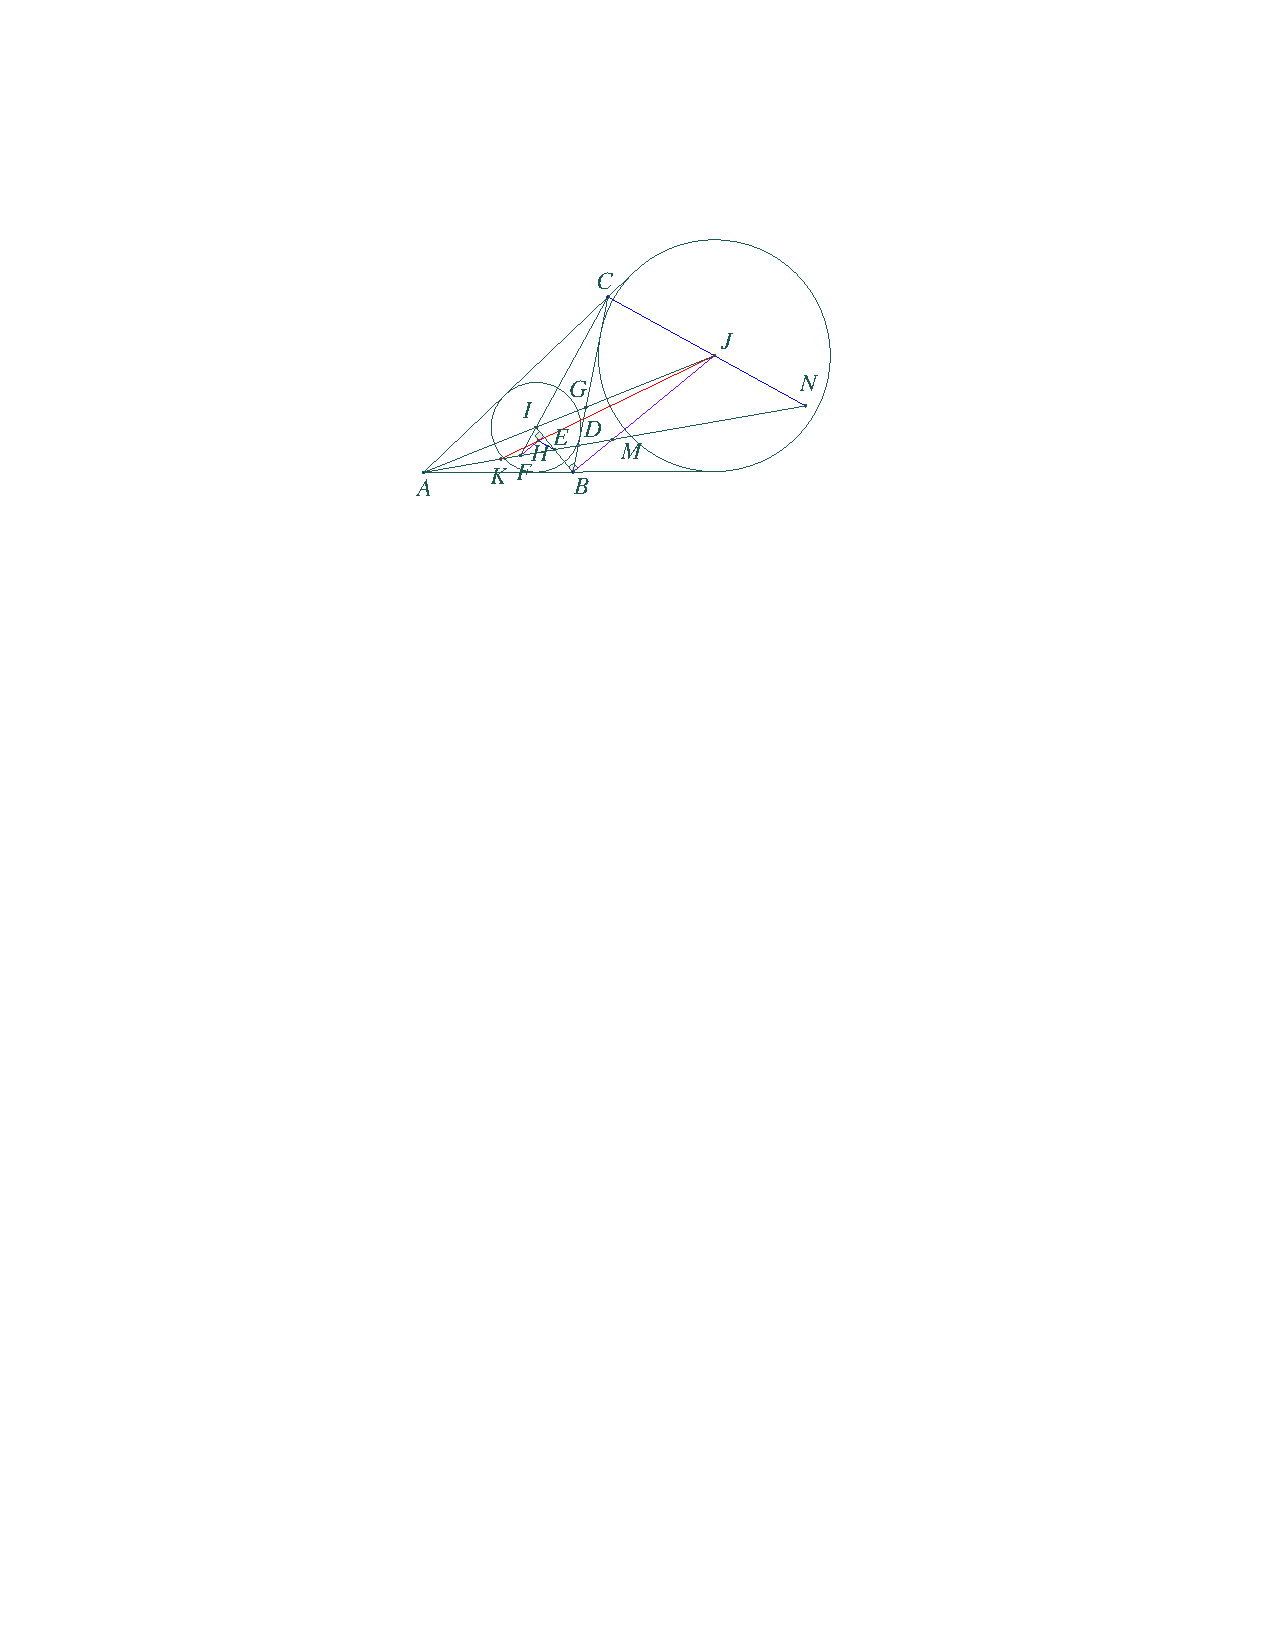
\includegraphics[width= 1\linewidth]{P738}
%		\caption{\small\textit{\color{}}}
		\vspace*{-10pt}
	\end{figure}
	Do $I$ là tâm đường tròn nội tiếp và $J$  là tâm đường tròn bàng tiếp góc $A$ của tam giác $ABC$, nên $BI$, $BJ$ tương ứng là phân giác trong, phân giác ngoài của góc $ABG$. Do đó, $IB \bot BJ$, và  $\left( {AGIJ} \right) =  - 1.$ Từ đây, do phép chiếu xuyên tâm bảo toàn tỷ số kép, nên
	
	Vì thế, do $K$ là trung điểm của $AD$, nên theo hệ thức Newton, ta có:
	\begin{align*}
		K{D^2} = \overline {KE}  \cdot \overline {KM} . \tag{$1$}
	\end{align*}
	Bằng cách tương tự, ta cũng chứng minh được
	\begin{align*}
		K{D^2} = \overline {KF}  \cdot \overline {KN} . \tag{$2$}
	\end{align*}
	Từ ($1$) và ($2$), suy ra
	\begin{align*}
		\overline {KE}  \cdot \overline {KM}  = \overline {KF}  \cdot \overline {KN} ;
	\end{align*}
	do đó, $\dfrac{{\overline {KE} }}{{\overline {KN} }} = \dfrac{{\overline {KF} }}{{\overline {KM} }}.$ \hfill ($3$)
	\vskip 0.05cm
	Đặt $\dfrac{{\overline {KE} }}{{\overline {KN} }} = k$;  và ký hiệu $f$ là phép vị tự tâm $K$, tỷ số $k$.
	\vskip 0.05cm
	Từ ($3$) suy ra, $f$ biến điểm $N$ thành điểm $E$, và biến điểm $M$ thành điểm $F$. \hfill ($4$)
	\vskip 0.05cm
	Tiếp theo, do $H$ là trực tâm tam giác $IEF$ (giả thiết) nên $FH \bot IE$, hay $FH \bot IB$ (do $I$, $E$, $B$ thẳng hàng). Mà $BJ \bot IB$ (chứng minh trên), hay $MJ \bot IB$ (do $M, B, J$ thẳng hàng), nên $FH \parallel MJ$.   \hfill     ($5$)
	\vskip 0.05cm
	Bằng cách hoàn toàn tương tự, ta cũng chứng minh được $EH \parallel NJ$.  \hfill   ($6$)
	\vskip 0.05cm
	Từ ($4$), ($5$) và ($6$) suy ra, $f$ biến đường thẳng $MJ$ thành đường thẳng $FH$, và biến đường thẳng $NJ$ thành đường thẳng $EH$. Do đó, $f$ biến điểm $J$ thành điểm $H$. Mà $K$ là tâm của $f$, nên $K, J, H$ thẳng hàng. Ta có điều phải chứng minh theo yêu cầu đề bài.
	\vskip 0.05cm
	\textbf{\color{thachthuctoanhoc}Bình luận và Nhận xét}
	\vskip 0.05cm
	$\pmb{1.}$ Lời giải trên cho thấy, kết luận của bài ra vẫn đúng, khi thay giả thiết ``$D$ thuộc cạnh $BC$, sao cho $A$, $I$, $D$ không thẳng hàng" bởi giả thiết ``$D$ thuộc đường thẳng $BC$, sao cho $A$, $I$, $D$ không thẳng hàng".
	\vskip 0.05cm
	$\pmb{2.}$ Tất cả các lời giải Tạp chí nhận được từ bạn đọc là lời giải đúng.
	\begin{flushright}
		\textbf{\color{thachthuctoanhoc}Hạ Vũ Anh}
	\end{flushright}
	{\color{thachthuctoanhoc}{\usefont{T5}{qag}{b}{n} P739.}}
	(Mức $A$) Cho dãy số $\left(a_n\right)$  xác định bởi
	\begin{align*}
		{a_n} = \left\lfloor {\frac{n}{{\sqrt 2 }}} \right\rfloor  + \left\lfloor {\frac{n}{{\sqrt 3 }}} \right\rfloor , \text{ với mọi } n \in \mathbb{N^*}.
	\end{align*}
	Chứng minh rằng, trong dãy $\left(a_n\right)$  có vô hạn số chẵn và vô hạn số lẻ.
	\vskip 0.1cm
	($\left\lfloor x \right\rfloor $  ký hiệu số nguyên lớn nhất không vượt quá $x$.)
	\vskip 0.05cm
	\textbf{\color{thachthuctoanhoc}Lời giải} (\textit{dựa trên ý tưởng của bạn Huỳnh Nguyễn Khánh Duy, lớp $12$ Toán, trường THPT chuyên Tiền Giang, tỉnh Tiền Giang})\textbf{\color{thachthuctoanhoc}.}
	\vskip 0.05cm
	Ta có Nhận xét sau:
	\vskip 0.05cm
	\textit{Nhận xét.} Với mọi  $x,y \in \mathbb{R}$, do $x - 1 < \left\lfloor x \right\rfloor  \le x$  và $y - 1 < \left\lfloor y \right\rfloor  \le y,$  nên
	\begin{align*}
		x - y - 1 < \left\lfloor x \right\rfloor  - \left\lfloor y \right\rfloor  < x - y + 1.
	\end{align*}
	Với mỗi $n \in \mathbb{N^*}$  đặt
	\begin{align*}
		&{u_n} = \left\lfloor {\frac{{n + 1}}{{\sqrt 2 }}} \right\rfloor  - \left\lfloor {\frac{n}{{\sqrt 2 }}} \right\rfloor \\
		\text{ và } &{v_n} = \left\lfloor {\frac{{n + 1}}{{\sqrt 3 }}} \right\rfloor  - \left\lfloor {\frac{n}{{\sqrt 3 }}} \right\rfloor .
	\end{align*}  
	Theo Nhận xét, với mọi $n \in \mathbb{N^*}$  ta có:
	\begin{align*}
		&- 1 + \frac{1}{{\sqrt 2 }} = \frac{{n + 1}}{{\sqrt 2 }} - \frac{n}{{\sqrt 2 }} - 1 \\
		< &{u_n} < \frac{{n + 1}}{{\sqrt 2 }} - \frac{n}{{\sqrt 2 }} + 1 = 1 + \frac{1}{{\sqrt 2 }};
	\end{align*}
	mà $u+n \in \mathbb{Z}$  nên $u_n \in \{0;1\}$  với mọi  $n \in \mathbb{N^*}$ \hfill ($1$)
	\vskip 0.05cm
	Bằng cách hoàn toàn tương tự, ta cũng chứng minh được: $v_n \in \{0;1\}$,  với mọi \linebreak$n \in \mathbb{N^*}$ \hfill     ($2$)
	\vskip 0.05cm
	Xét số nguyên dương $k$ tùy ý.
	\vskip 0.05cm
	Theo Nhận xét, ta có:
	\begin{align*}
		\sum\limits_{i = k}^{k + 100} {{u_i}}  &= \sum\limits_{i = k}^{k + 100} {\left( {\left\lfloor {\frac{{i + 1}}{{\sqrt 2 }}} \right\rfloor  - \left\lfloor {\frac{i}{{\sqrt 2 }}} \right\rfloor } \right)}  \\
		&= \left\lfloor {\frac{{k + 101}}{{\sqrt 2 }}} \right\rfloor  - \left\lfloor {\frac{k}{{\sqrt 2 }}} \right\rfloor  \\
		&> \frac{{k + 101}}{{\sqrt 2 }} - \frac{k}{{\sqrt 2 }} - 1 = \frac{{101}}{{\sqrt 2 }} - 1 \\
		&> 70, \tag{$3$}\\
		\sum\limits_{i = k}^{k + 100} {{v_i}}  &= \sum\limits_{i = k}^{k + 100} {\left( {\left\lfloor {\frac{{i + 1}}{{\sqrt 3 }}} \right\rfloor  - \left\lfloor {\frac{i}{{\sqrt 3 }}} \right\rfloor } \right)}  \\
		&= \left\lfloor {\frac{{k + 101}}{{\sqrt 3 }}} \right\rfloor  - \left\lfloor {\frac{k}{{\sqrt 3 }}} \right\rfloor \\
		& < \frac{{k + 101}}{{\sqrt 3 }} - \frac{k}{{\sqrt 3 }} + 1 = \frac{{101}}{{\sqrt 3 }} + 1\\
		& < 60. \tag{$4$}
	\end{align*}
	Từ ($1$) và ($3$) suy ra, trong $101$ số ${u_k},{u_{k + 1}}, \ldots ,{u_{k + 100}}$  có ít nhất $71$ số bằng $1$.
	\vskip 0.05cm
	Từ ($2$) và ($4$) suy ra, trong $101$ số ${v_k},{v_{k + 1}}, \ldots ,{v_{k + 100}}$  có tối đa $59$ số bằng $1$.
	\vskip 0.05cm
	Vì vậy, tồn tại $m \in \{k; k + 1; \ldots; k + 100\}$ sao cho $u_m = 1$  và $v_m = 0$.
	\vskip 0.05cm 
	Ta có:
	\begin{align*}
		&{a_{m + 1}} - {a_m}\\
		= &\left\lfloor {\frac{{m + 1}}{{\sqrt 2 }}} \right\rfloor  + \left\lfloor {\frac{{m + 1}}{{\sqrt 3 }}} \right\rfloor  - \left\lfloor {\frac{m}{{\sqrt 2 }}} \right\rfloor  - \left\lfloor {\frac{m}{{\sqrt 3 }}} \right\rfloor  \\
		= \,\,&{u_m} + {v_m} = 1.
	\end{align*}
	Suy ra, ${a_m}\not  \equiv {a_{m + 1}}\left( {\bmod 2} \right).$  Từ đây, do tính tùy ý của số nguyên dương $k$, suy ra, trong $101$ số hạng liên tiếp tùy ý của dãy $\left(a_n\right)$  luôn có đồng thời cả số chẵn và số lẻ. Mà $\left(a_n\right)$  là dãy vô hạn, nên trong dãy đó có vô hạn số chẵn và vô hạn số lẻ. Ta có điều phải chứng minh theo yêu cầu đề bài.
	\vskip 0.05cm
	\textbf{\color{thachthuctoanhoc}Bình luận và Nhận xét}
	\vskip 0.05cm
	Lời giải của bạn \textit{Huỳnh Nguyễn Khánh Duy} là lời giải duy nhất Tạp chí nhận được từ bạn đọc, và là một lời giải đúng.
	\begin{flushright}
		\textbf{\color{thachthuctoanhoc}Lưu Thị Thanh Hà}
	\end{flushright}
	{\color{thachthuctoanhoc}{\usefont{T5}{qag}{b}{n} P740.}}
	(Mức $A$) Cho bảng ô vuông kích thước $2023 \times 2023$. Tìm số nguyên dương $n$ nhỏ nhất, sao cho có thể đặt $n$ viên bi vào các ô vuông con của bảng, đảm bảo các điều kiện sau được đồng thời thỏa mãn:
	\vskip 0.05cm
	$i/$ Ở mỗi ô vuông con chỉ có tối đa một viên bi;
	\vskip 0.05cm
	$ii/$ Với mỗi ô vuông con không có bi, tổng số viên bi ở hàng và cột chứa ô đó không nhỏ hơn $2023$.
	\vskip 0.05cm
	\textbf{\color{thachthuctoanhoc}Lời giải} (\textit{dựa theo cách giải của bạn Nguyễn Gia Khánh, lớp $12$ Toán $1$, trường THPT chuyên Hưng Yên, tỉnh Hưng Yên})\textbf{\color{thachthuctoanhoc}.}
	\vskip 0.05cm
	Đánh số thứ tự các hàng của bảng đã cho, từ trên xuống dưới, lần lượt bởi $1, 2, \ldots, 2023$; và đánh số thứ tự các cột của bảng đó, từ trái qua phải, lần lượt bởi $1, 2, \ldots, 2023$.
	\vskip 0.05cm
	Với mỗi $i \in  \{1; 2; \ldots; 2023\}$, ta gọi hàng được đánh số thứ tự $i$ là hàng $i$, và gọi cột được đánh số thứ tự $i$ là cột $i$.
	\vskip 0.05cm
	Với $i, j \in \{1; 2; \ldots; 2023\}$, ký hiệu ô vuông con nằm ở giao của hàng thứ $i$ và cột thứ $j$ bởi $(i, j)$.
	\vskip 0.05cm
	Giả sử $n$ là số nguyên dương sao cho có thể đặt $n$ viên bi vào các ô vuông con của bảng, đảm bảo các điều kiện $i/$ và $ii/$ được đồng thời thỏa mãn.
	\vskip 0.05cm
	Xét một cách đặt bi tùy ý, thỏa mãn các yêu cầu của đề bài.
	\vskip 0.05cm
	Với mỗi $i \in \{1; 2; \ldots; 2023\}$, gọi $a_i$  là số viên bi được đặt vào hàng $i$, và  $b_i$ là số viên bi được đặt vào cột $i$.
	\vskip 0.05cm
	Do tổng số viên bi được đặt vào bảng bằng $n$, nên
	\begin{align*}
		\sum\limits_{i = 1}^{2023} {{a_i}}  = \sum\limits_{i = 1}^{2023} {{b_i}}  = n. \tag{$1$}
	\end{align*}
	Đặt $m = 2023^2 -n$ \hfill    ($2$)
	\vskip 0.05cm
	Do số bi ở mỗi ô tối đa là $1$ và trong bảng có $n$ viên bi, nên trong bảng có đúng $n$ ô có bi. Vì thế, trong bảng có đúng $m$ ô không có bi. Giả sử các ô này là $(p_1,q_1), (p_2,q_2), \ldots, (p_m,q_m)$.
	\vskip 0.05cm 
	Theo giả thiết của bài ra, với mọi $i \in \{1; 2; \ldots; m\}$, đều có
	\begin{align*}
		{a_{{p_i}}} + {b_{{q_i}}} \ge 2023. \tag{$3$}
	\end{align*}
	Với mỗi $k \in \{1; 2; \ldots; 2023\}$, do trong hàng $k$ có đúng $2023 - a_k$  ô không có bi, và trong cột $k$ có đúng $2023-b_k$  ô không có bi, nên số $k$ xuất hiện đúng $2023- a_k$  lần trong dãy $p_1,p_2,\ldots,p_m$  và xuất hiện đúng $2023-b_k$  lần trong dãy $q_1, q_2,\ldots,q_m$.
	\vskip 0.05cm 
	Vì vậy
	\begin{align*}
		\sum\limits_{i = 1}^m {{a_{{p_i}}}} & = \sum\limits_{k = 1}^{2023} {\left( {2023 - {a_k}} \right){a_k}} \\
		& = 2023 \cdot \sum\limits_{k = 1}^{2023} {{a_k}}  - \sum\limits_{k = 1}^{2023} {a_k^2}  \\
		&= 2023 \cdot n - \sum\limits_{k = 1}^{2023} {a_k^2} \quad\text{(do ($1$))}; \tag{$4$}\\
		\sum\limits_{i = 1}^m {{b_{{q_i}}}}  &= \sum\limits_{k = 1}^{2023} {\left( {2023 - {b_k}} \right){b_k}}  \\
		&= 2023 \cdot \sum\limits_{k = 1}^{2023} {{b_k}}  - \sum\limits_{k = 1}^{2023} {b_k^2}  \\
		&= 2023 \cdot n - \sum\limits_{k = 1}^{2023} {b_k^2} \quad\text{(do ($1$))}. \tag{$5$}
	\end{align*}
	Từ ($3$), ($4$) và ($5$), với lưu ý tới ($2$), suy ra
	\begin{align*}
		&2023\left( {{{2023}^2} - n} \right) \le \sum\limits_{i = 1}^m {\left( {{a_{{p_i}}} + {b_{{q_i}}}} \right)}  \\
		= \,&2 \cdot 2023n - \sum\limits_{k = 1}^{2023} {\left( {a_k^2 + b_k^2} \right)} .
	\end{align*}
	Do đó
	\begin{align*}
			3 \cdot 2023n &\ge {2023^3} + \sum\limits_{k = 1}^{2023} {\left( {a_k^2 + b_k^2} \right)}  \\
			&\ge {2023^3} + \sum\limits_{k = 1}^{2023} {\frac{{{{\left( {{a_k} + {b_k}} \right)}^2}}}{2}} \\
			 &\ge {2023^3} + \frac{{{{\left( {\sum\limits_{k = 1}^{2023} {\left( {{a_k} + {b_k}} \right)} } \right)}^2}}}{{2 \cdot 2023}} \\
			 &= {2023^3} + \frac{{{{\left( {2n} \right)}^2}}}{{2 \cdot 2023}} \quad\left( {{\rm{do}}(1)} \right).
	\end{align*}
	Suy ra
	\begin{align*}
		2{n^2} - 3 \cdot {2023^2} \cdot n + {2023^4} \le 0.
	\end{align*}
	Vì vậy
	\begin{align*}
		n \ge \frac{{{{2023}^2}}}{2} &= \frac{{2\left( {{{1011}^2} + {{1012}^2}} \right) - 1}}{2} \\
		&= {1011^2} + {1012^2} - \frac{1}{2}.
	\end{align*}
	Từ đó, do $n \in \mathbb{N^*}$,  suy ra  $n \ge {1011^2} + {1012^2}$.
	\vskip 0.05cm
	Xét cách đặt $1011^2 + 1012^2$  viên bi vào bảng, như sau:
	\vskip 0.05cm
	Đặt vào mỗi ô vuông con của bảng con $1011 \times 1011$, tạo bởi các hàng $1, 2, \ldots, 1011$ và các cột $1, 2, \ldots, 1011$, một viên bi; và đặt vào mỗi ô vuông con của bảng con $1012 \times 1012$, tạo bởi các hàng $1012, 1013, \ldots, 2023$ và các cột $1012, 1013, \ldots, 2023$, một viên bi.
	\vskip 0.05cm
	Dễ thấy, ở cách đặt trên, với mỗi ô vuông con không có bi, tổng số viên bi ở hàng và cột chứa ô đó đúng bằng $2023$. Vì thế, cách đặt đó thỏa mãn tất cả các điều kiện của đề bài.
	\vskip 0.05cm
	Vậy, $n = 1011^2 + 1012^2$ là số nguyên dương nhỏ nhất thỏa mãn yêu cầu đề bài.
	\vskip 0.05cm
	\textbf{\color{thachthuctoanhoc}Bình luận và Nhận xét}
	\vskip 0.05cm
	$\pmb{1.}$ Có thể phát biểu bài đã ra một cách đơn giản hơn, như sau:
	\vskip 0.05cm
	``Cho bảng ô vuông kích thước $2023 \times 2023$. Tìm số nguyên dương $n$ nhỏ nhất, để có thể đánh dấu $n$ ô vuông con của bảng, sao cho với mỗi ô vuông con không được đánh dấu, tổng số ô được đánh dấu ở hàng và cột chứa ô đó không nhỏ hơn $2023$."
	\vskip 0.05cm
	$\pmb{2.}$ Trong số các lời giải Tạp chí nhận được từ bạn đọc, lời giải của bạn \textit{Nguyễn Gia Khánh} là lời giải đúng duy nhất; các lời giải còn lại đều mắc lỗi thiếu kiểm tra cách đặt $1011^2 + 1012^2$ viên bi, đã chỉ ra ở lời giải, thỏa mãn các điều kiện của đề bài.
	\begin{flushright}
		\textbf{\color{thachthuctoanhoc}Nguyễn Khắc Minh}
	\end{flushright}
\end{multicols}
